%--------------------------------------------------------------------------------------------------
% 
\chapter{Introduction}
%--------------------------------------------------------------------------------------------------

%\section{Motivation}
In this section, we briefly explore the significance of cross-lingual news analysis in the Slovene language for the Natural Language Processing (NLP) field and provide the motivation behind this paper.

\section{News Monitoring and Analysis}
Initially, the purpose of News monitoring and analysis was to relieve us from monitoring all published news; however, as the volume of news increased, it had to evolve and employ more advanced Natural Language Processing (NLP) techniques.
News Monitoring and analysis can positively influence society because its objective is to present and analyse all news content impartially without favouring any particular viewpoint. 
Additionally, it benefits society by striving to identify biased perspectives, misinformation and sentiment within news content.
Nowadays, media monitoring and analysis must be conducted in real-time, which involves organising articles based on their content, attaching various metadata categories, and synthesising information from multiple news sources.
Natural Language Processing (NLP) techniques can effectively address these challenges by facilitating the development of personalised news recommendation systems, automated content summarisation, organising and prioritising news items, and ensuring users access the most pertinent and up-to-date information.
These tools allow users to quickly glean the essential information from an article, saving time and reducing cognitive load.

\begin{figure}
  \centering
  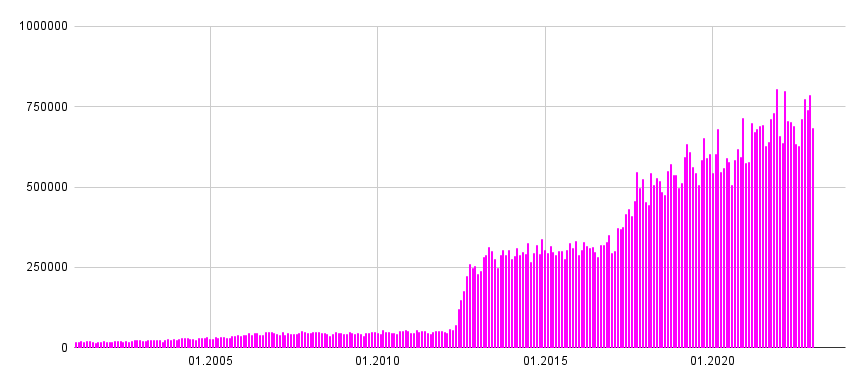
\includegraphics[width=0.7\textwidth]{figures/articles.png}
  \caption{Increasing number of client-relevant news articles in the Balkan region monitored by the industry.}
  \label{fig:sl_predictions}
\end{figure}

\section{NLP, Slovene and Other South Slavic Languages}
Creating solutions for under-resourced languages is crucial in increasing the presence of non-dominant languages within the digital realm.
The western Balkan region, formerly also a common political entity, has common cultural and language origins. 
This allows us to explore also the possibilities of transfer learning in NLP between languages from the same family where training resources are scarce. 
The accessibility of annotated training materials for the Slovene language has experienced significant enhancement, thanks to the efforts of Common Language Resources and Technology Infrastructure, Slovenia~\parencite{clarin_si} and The Jožef Stefan Institute~\parencite{nl_ijs_si}. 
However, the size of training corpora for other South Slavic languages remains limited or, in some cases, absent.
Additionally, Slovene and other South Slavic languages pose unique challenges in NLP since they are highly inflected, with a rich system of inflectional morphology for nouns, pronouns, adjectives, and verbs.

\section{Cross-Lingual NLP Techniques}

The main objective of cross-lingual NLP is to transfer knowledge from high-resource languages to low-resource languages where training data size is small or nonexistent.
Fundamental techniques in the cross-lingual setting include multilingual pre-training, transfer learning, and zero-shot learning.

\subsection{Large Pretrained Multilingual Models}

Within Natural Language Processing, Transformer-based~\parencite{vaswani2017attention} deep neural networks have recently emerged as the prevailing approach.
Large pre-trained multilingual language models (LPMLMs), such as mBERT~\parencite{devlin2018bert} and XLM-RoBERTa~\parencite{conneau2019xlmr}, can solve nearly all linguistic tasks (e.g., information extraction, text classification, sentiment analysis, topic detection, etc.) better compared to conventional NLP techniques. 
LPMLMs are initially trained on unsupervised, broad corpora but can be fine-tuned for particular tasks, such as sequence or token classification.

The language model learned in pre-training reduces the amount of labelled data needed for fine-tuning.
This is more than evident in the recent advancements of the text-to-text transformers like T5~\parencite{raffel2020exploring}, Generative Pretrained Transformer (GPT) family~\parencite{brown2020language}, PaLM~\parencite{chowdhery2022palm}, and LLama~\parencite{touvron2023llama}, which are fine-tuned on a wide range of text-based tasks, including question-answering, text generation, and language translation to name a few.

Various experiments also achieved state-of-the-art performance in specific NLP tasks for the Slovene language. 
For instance, sentiment analysis~\parencite{pelicon2020zero}, keyword extraction~\parencite{martinc2021tntkid}, named entity recognition~\parencite{prelevikj-zitnik-2021-multilingual}, cross-lingual hate-speech detection \parencite{pelicon2021offensive}, etc.
All state-of-the-art NLP techniques presented in this paper use Transformer-based neural network architecture as its foundation.

\subsection{Zero-shot and Few-shot Learning}

The Zero-shot technique, first used in classification tasks with a target to predict new unseen classes~\parencite{chang2008zero, larochelle2008zero, palatucci2009zero}, has broadened its meaning by use in various NLP tasks.
The Zero-shot term (and technique) is also used as a cross-lingual model transfer in which task-specific annotations in one language are used to fine-tune the model for evaluation in another language~\parencite{pires2019multilingual}. Zero-shot cross-lingual model transfer use was also demonstrated from Slovene to Croatian language~\parencite{pelicon2020zero}.

Until recently, task-specific fine-tuning was a prevailing method of achieving state-of-the-art results in NLP. 
GPT models have shown unprecedented performance in Zero-shot and Few-shot Learning, as was shown by \textcite{brown2020language}.
Active research is being conducted on different architectures and pre-training objectives used in state-of-the-art models. 
\textcite{Wang2022WhatLM} demonstrated that the masked language objective with encoder-decoder architecture works best for Zero-shot NLP learning after multi-task fine-tuning. In contrast, \textcite{touvron2023llama} showed that the text-to-text transformer model can be much smaller (than GPT) and still competitive.


\section{Evaluation Metrics}

This section discusses quantitative evaluation measures for Named Entity Recognition (NER) and Computational Framing Analysis (CFA).
Traditionally, NER is modelled as a multi-class classification problem, whereas CFA has recently been more commonly viewed as a multi-label classification problem.
Therefore macro-averaged F1-score over all classes is used for NER, while for CFA, micro-averaged F1-score and Hamming Loss over all labels are also often used~\parencite{yang2018sgm}.
Macro-averaged F1-score is commonly used to evaluate CFA model performance when exactly one frame is to be predicted.

\subsection{F-measure}

Traditionally, an F-measure or balanced F-score is used to evaluate the classification models.
F-score is the harmonic mean of precision and recall and can have values between 0 and 1 (closer to 1 means a better score):
\begin{equation*}
    \text{F1-score} = 2  \cdot \frac{Precision \cdot Recall}{Precision +  Recall}
\end{equation*}
The Precision and Recall are defined as:
\begin{equation*}
\begin{split}
    \text{Precision} = \frac{TP}{TP + FP}
\end{split}
\quad\quad
\begin{split}
    \text{Recall} = \frac{TP}{TP + FN}
\end{split}
\end{equation*}
given that:
\begin{itemize}
  \item False Positives (FP): a class or label predicted but not present in the test.
  \item False Negatives (FN): a class or label is present in the test but missing in our prediction.
  \item True Positives (TP): a class or label that is correctly predicted.
  \item True Negatives (TN): a class or label that is correctly not predicted and not present in the test.
\end{itemize}

\subsection{Macro F-scores}

Macro-averaged F1-score is computed using the arithmetic mean of all the per-class $F1_i$ scores:
\begin{equation*}
    \text{Macro-averaged F1-score} = \frac{1}{n}\sum_{i=1}^{n} F1_i
\end{equation*}
where $F1_i$ is the F1-score for $ith$ label or class.

\subsection{Micro F-scores}
Micro-averaging calculates a global average F1 score by aggregating the counts of True Positives ($TP_a$), False Negatives ($FN_a$), and False Positives ($FP_a$) for all classes or labels. Micro-averaged F1-score can then be derived from Precision and Recall equations:

\begin{equation*}
    \text{Micro-averaged F1-score} = \frac{TP_a}{TP_a + \frac{1}{2}(FP_a+FN_a)}
\end{equation*}

\subsection{Accuracy}
The accuracy of the classification model is commonly represented as a fraction of correctly classified predictions overall predictions. 
In multi-class classification cases where each observation has a single label, the micro-F1 and accuracy share the same value, but in general, we can define accuracy as:
\begin{equation*}
    \text{Accuracy} = \frac{TP_a + TN_a}{TP_a + FP_a + FN_a + TN_a)}
\end{equation*}

\subsection{Hamming-loss}

Hamming loss is a common multi-label evaluation metric defined as the fraction of the wrong labels to the total number of labels.

\begin{equation*}
    \text{Hamming loss} = \frac{1}{n \cdot l}\sum_{i=1}^{n}\sum_{j=1}^{l}{xor(y_i,\hat{y_i})}
\end{equation*}
where $n$ is the number of samples, $l$ is the number of labels, $y_i$ is the target, $\hat{y_i}$ is the prediction, and $xor$ is exclusive or operator that returns zero when the target and prediction are identical and one otherwise.

\begin{table}[htb]
    \caption{Example Hamming loss calculation: $\frac{5}{4 \cdot 5} = 0.25$ where each row contains a target $y_i$ followed by a prediction $\hat{y_i}$ vector with five label values with five wrong predictions in total}
	\label{tab:hamming}
	\centering
    \begin{tabular}{lll}
        \hline
        &$y_i$&$\hat{y_i}$\\
        \hline
        $x_1$&$[1, 0, 1, 1, 0]$&$[1, 0, 1, \textcolor{red}{0}, \textcolor{red}{1}]$\\
        $x_2$&$[0, 1, 1, 0, 0]$&$[0, 1, 1, \textcolor{red}{1}, 1]$\\
        $x_3$&$[0, 0, 0, 1, 0]$&$[0, 0, \textcolor{red}{1}, 1, \textcolor{red}{1}]$\\
        $x_4$&$[1, 1, 0, 1, 0]$&$[1, 1, 0, 1, 0]$\\
        \hline
    \end{tabular}
\end{table}

Contrary to F-score, a Hamming loss closer to 0 means a better score.


\section{Scope and Objectives}
The scope of this paper is to present two common NLP tasks and their state-of-the-art, Named Entity Recognition (NER) and Computational Framing Analysis (CFA). 
NER has a long history and is one of the most common NLP tasks that can be used for news analysis. 
CFA gained traction in NLP in recent years, where more and more emphasis is given to the analysis of implicit suggestion or persuasion in text.
Both topics will be presented in the context of news analysis with a strong emphasis on the Slovene and other Slavic languages, where cross-lingual techniques are sometimes the only option to tackle the given problem. 
For the CFA, we consider the state-of-the-art in other languages since we conducted only preliminary research in Zero-shot learning for the Slovene language.

\section{Organization of the Paper}

In the following chapter, we introduce NER, including its annotation methods and a concise history of NER research. 
We then explore the latest advancements in NER for the Slovene language and conclude with an overview of the training datasets.

In Chapter~\ref{ch:nfa}, we first present the CFA and its research history. 
Next, we discuss the current state-of-the-art in CFA.
Finally, we conclude the chapter by exploring the available datasets and briefly outlining our initial research findings.

In conclusion, we critically analyse both NER and CFA topics, followed by a discussion of potential enhancements and an outline of our planned research endeavours for the future.